
%-----Chapter 2: Simulation-------%
\chapter{Simulation}

One main aspect of this group work among the design of a Kalman filter was the construction of a graphical environment for our work, so we decided to implement a simulation of a Nao soccer match in MATLAB. Therefore we created three independent modules which build the framework for the simulation. The three parts contain functions concerning the playing field, the robots and the ball respectively. Since these parts are constructed in a modular fashion, we can change one module without influencing the other two.


\section{The Playing Field}

All graphical features concerning the playing field are implemented by the function {\fontfamily{pcr}\selectfont plot\_env(ball).m}. As you can see the graphics of the ball are also part of this function. The reason why we didn't need a seperate function for the ball is that the appearance of the ball, contrary to this of the robots, always stays the same. The function {\fontfamily{pcr}\selectfont plot\_env(ball).m} itself is again subdivided in three functions, which draw the field, the ball and, as a neat add on, the scorecounter seperately. We mostly use built-in MATLAB commands for this task such as {\fontfamily{pcr}\selectfont rectangle()} or {\fontfamily{pcr}\selectfont line()}. The following short code excerpt shows for example how the center point of the playing field is drawn

\lstinputlisting[firstline=27, lastline=28]{../Simulation/Merge/plot_env.m}
\parskip 20pt

where {\fontfamily{pcr}\selectfont draw\_circle(x,y,r,color,filled)} is a custom-build function to draw marker circles of the field, but also circles representing the robots and the ball. All functions are designed for fast calculations since we want as many frames as possible if the simulation is running. Figure \ref{KFchart} shows the playing field after the execution of {\fontfamily{pcr}\selectfont plot\_env(ball).m} with suitable parameters for {\fontfamily{pcr}\selectfont ball}
\parskip 10pt

\begin{figure}[htbp]
	\centering
    	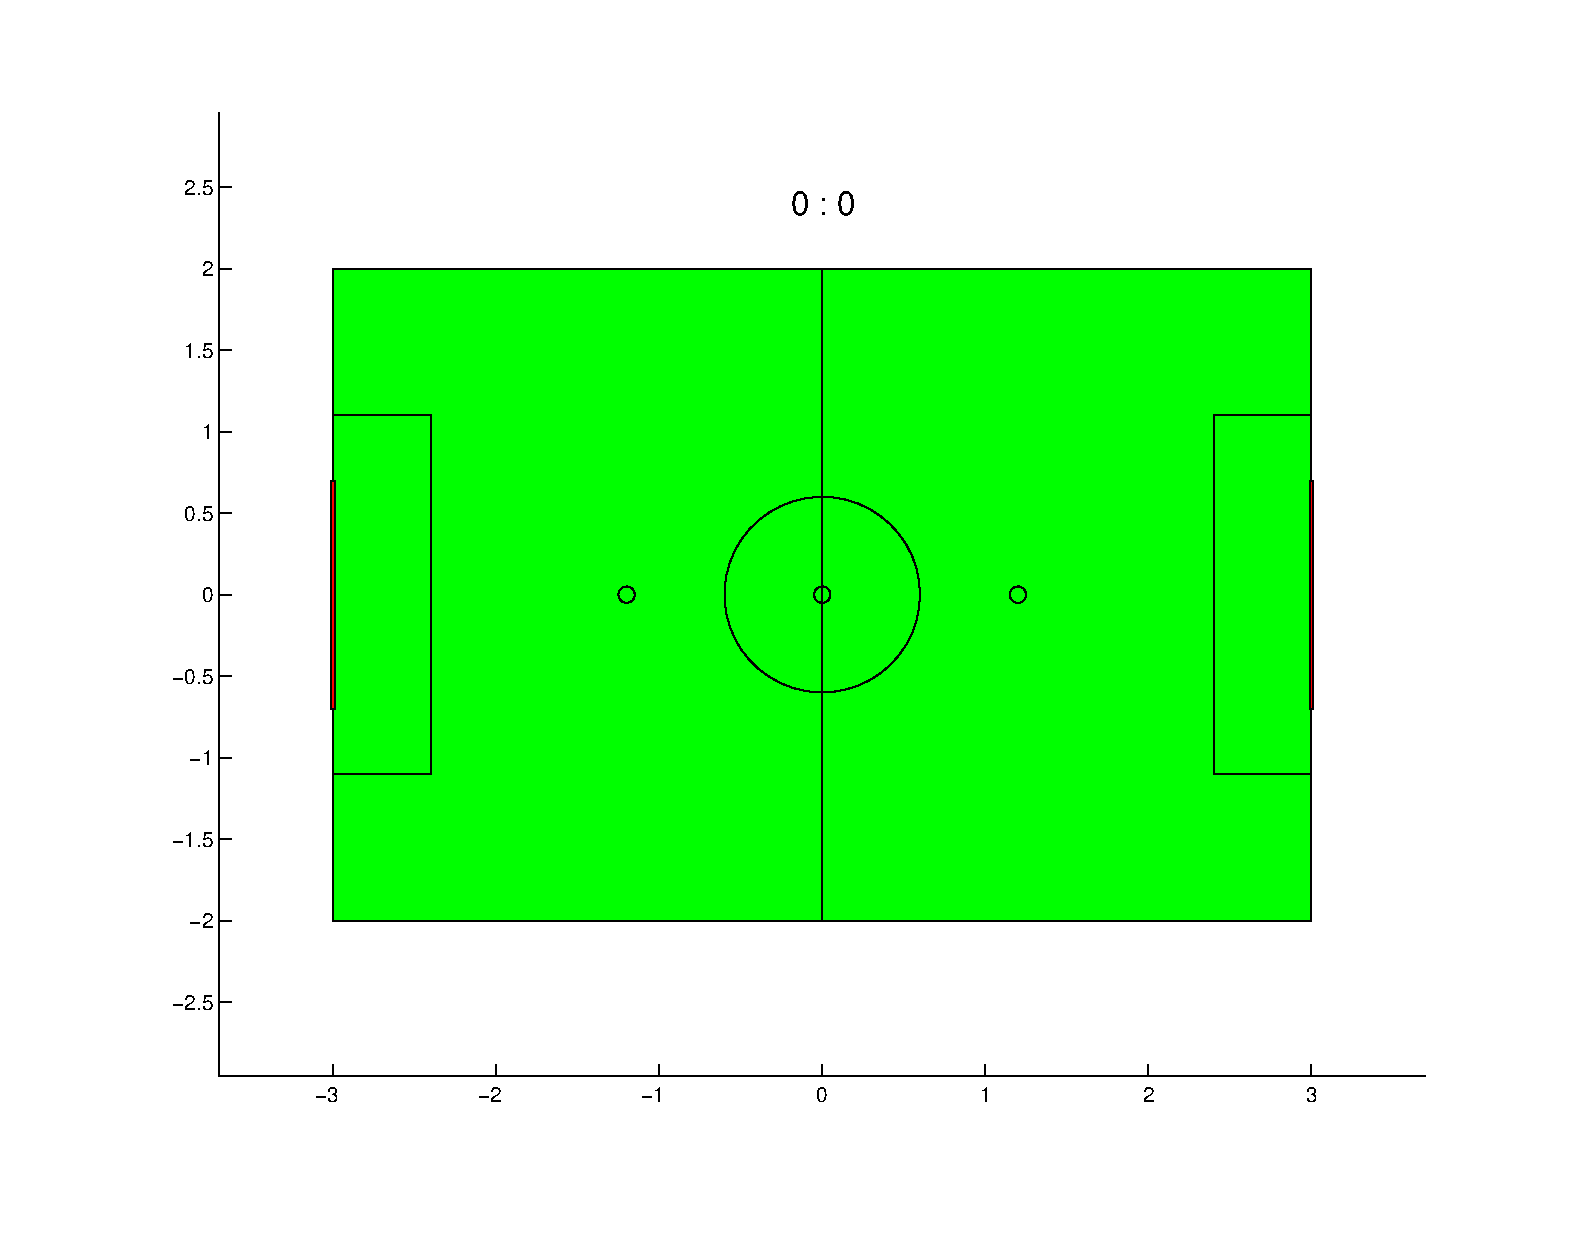
\includegraphics[width=12cm]{./2_Simulation/playing_field}
  	\caption{Playing field after initialization.}
  	\label{KFchart}
\end{figure}


\section{The Robots}

Maybe the most important part of the simulation is the adequate depiction and behaviour of all eight robots. The latter task is split in three components: In a first step the robots are initialized, after that, their new positions on the field, according to their motion equations, are computed and in the end we are adding measurement noise for our filtering task. The initialization of the robots is quite simple. The function {\fontfamily{pcr}\selectfont dummy\_init().m} just creates eight structs with the essential informations for every robot, i.e. its horizontal and vertical position, its direction and its team affiliation. Furthermore the function defines the robot's radius and its maximum possible angular change for one timestep as global variables. In a latter stage of development we dropped the simplification of a global eye and assumed that a location of a robot's position is only possible if it is in the sight of view of at least one other robot. So in the second version {\fontfamily{pcr}\selectfont robot\_init().m} of this function, we additionally defined global variables for the robot's velocity, its distance of sight as well as its angle of sight. Once initialized we use the functions {\fontfamily{pcr}\selectfont dummy\_step(Robot).m} and {\fontfamily{pcr}\selectfont robot\_step(Robot).m} respectively to compute the attributes of all robots for every timestep. The key issue of both functions however is the recalculation of the position, i.e. the motion of the robots

\lstinputlisting[firstline=20, lastline=27]{../Simulation/Merge/dummy_step.m}
\parskip 20pt

Later on this non-linearity of these equations will make it necessary that we use an extended Kalman filter instead of a simple linear one. The addition of process noise and the collision detection of robots also happen in these functions. Up to this point we computed the behaviour of an ideal robot. Since our goal is to filter out the uncertainty of motion of the robot parameters, we artifically have to add some measurement noise which we can filter later on. The functions {\fontfamily{pcr}\selectfont dummy\_measure(Robot).m} and {\fontfamily{pcr}\selectfont robot\_measure(Robot).m} are implemented for that purpose. {\fontfamily{pcr}\selectfont dummy\_measure(Robot).m} simply adds white Gaussian noise to the position and the direction of every robot. Additionally with a certain possibillity there is no measurement at all, so the corresponding parameter is dropped. What we are assuming with this model is, that there is some global eye available which measures the position and direction of every robot with some given resolution. Since this scenario is not realistic in a RoboCup soccer match, because only the robots themselves can gain visual information, we developed the function {\fontfamily{pcr}\selectfont robot\_measure(Robot).m} to solve this problem.



\parskip 10pt

\section{The Ball}



\section{A Random Simulation}

